% This file was created with tikzplotlib v0.10.1.
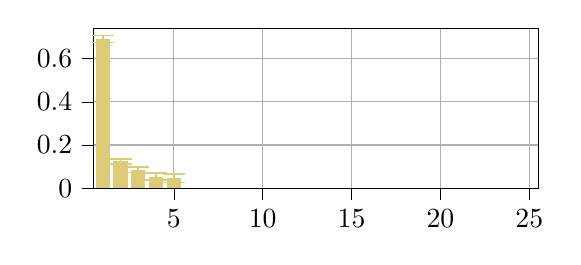
\begin{tikzpicture}

\definecolor{burlywood221204119}{RGB}{221,204,119}
\definecolor{darkgray176}{RGB}{176,176,176}

\begin{axis}[
height=1.4222438079424382in,
tick align=outside,
tick pos=left,
width=2.8444876158848764in,
x grid style={darkgray176},
xmajorgrids,
xmin=0.5, xmax=25.5,
xtick style={color=black},
y grid style={darkgray176},
ymajorgrids,
ymin=0, ymax=0.741468571001166,
ytick style={color=black}
]
\draw[draw=none,fill=burlywood221204119] (axis cs:0.6,0) rectangle (axis cs:1.4,0.691468571001166);
\draw[draw=none,fill=burlywood221204119] (axis cs:1.6,0) rectangle (axis cs:2.4,0.123694090759194);
\draw[draw=none,fill=burlywood221204119] (axis cs:2.6,0) rectangle (axis cs:3.4,0.0855952955071137);
\draw[draw=none,fill=burlywood221204119] (axis cs:3.6,0) rectangle (axis cs:4.4,0.0529272528936169);
\draw[draw=none,fill=burlywood221204119] (axis cs:4.6,0) rectangle (axis cs:5.4,0.0463147898389094);
\path [draw=burlywood221204119, semithick]
(axis cs:1,0.675122353633052)
--(axis cs:1,0.707814788369279);

\path [draw=burlywood221204119, semithick]
(axis cs:2,0.111138548115052)
--(axis cs:2,0.136249633403336);

\path [draw=burlywood221204119, semithick]
(axis cs:3,0.0717460052671802)
--(axis cs:3,0.0994445857470472);

\path [draw=burlywood221204119, semithick]
(axis cs:4,0.0368739029595636)
--(axis cs:4,0.0689806028276702);

\path [draw=burlywood221204119, semithick]
(axis cs:5,0.0256408689650123)
--(axis cs:5,0.0669887107128065);

\addplot [semithick, burlywood221204119, mark=-, mark size=4, mark options={solid}, only marks]
table {%
1 0.675122353633052
2 0.111138548115052
3 0.0717460052671802
4 0.0368739029595636
5 0.0256408689650123
};
\addplot [semithick, burlywood221204119, mark=-, mark size=4, mark options={solid}, only marks]
table {%
1 0.707814788369279
2 0.136249633403336
3 0.0994445857470472
4 0.0689806028276702
5 0.0669887107128065
};
\end{axis}

\end{tikzpicture}
